\section{Testing degli utenti}
\label{s:testing-utenti}

\subsection{Progettazione del test}
\label{ss:vd-progettazione-test}
Per testare la nostra riprogettazione, abbiamo ritenuto opportuno perseguire l'approccio Guerrilla (o Discount) usability testing già utilizzato nella \hyperref[s:verifica-risorse-esistenti-testing-utenti]{Sezione 2.3 Testing da parte degli utenti}.\\
In questo caso abbiamo però utilizzato una strategia di test di tipo formativa, in quanto il nostro obiettivo era quello di trovare quanti più problemi di usabilità possibili grazie agli utenti coinvolti nei test.\\
L'ambito del test è stato orizzontale, dal momento che il prodotto a nostra disposizione è un wireframe con interazioni sufficienti al solo scopo esemplificativo. In altre parole, le interazioni presenti sono volte a spiegare il funzionamento delle varie componenti grafiche, mentre non sempre permettono di portare a termine i task in un modo realistico.\\
Il setting in cui sono stati condotti i test ha visto l'utilizzo di software di videoconferenza. Gli assistenti del test siamo stati noi stessi, in qualità di membri del team di design. La selezione dei partecipanti è avvenuta mediante l'invio di una mail agli indirizzi dei giornalisti precedentemente contattati in occasione della ricerca etnografica e del testing sulle risorse esistenti.\\
I dati raccolti hanno natura qualitativa: in dettaglio, abbiamo chiesto ad ogni giornalista di simulare l'esecuzione di certi task mediante il wireframe e di esprimerci le sue impressioni a riguardo. L'output del test si è concretizzato, pertanto, in un insieme di dichiarazioni circa gli aspetti migliori dell'interfaccia progettata, nonché le criticità da risolvere.\\
Dato l'esiguo numero di giornalisti che si sono offerti per il test (tre) e la natura qualitativa dei dati raccolti, abbiamo deciso di analizzarli applicando il buon senso.\\
Per i task sottoposti a ciascun utente, abbiamo attinto da quelli già selezionati nella prima fase di testing sulle risorse esistenti:
\begin{enumerate}
    \item calcolare il tasso di positività (calcolato come il rapporto tra nuovi positivi e i tamponi effettuati) relativo al 17 novembre 2020\footnote{La data del 17 novembre 2020 è completamente casuale. Inoltre, avendo a disposizione un wireframe, si è chiesto al giornalista di simulare la selezione della data, senza effettivamente portarla a termine.};    
    \item valutare l'occupazione delle strutture sanitare al 17 novembre 2020;
    \item calcolare il tasso di letalità (calcolato come il rapporto tra il numero dei deceduti e il numero dei casi) medio nel mese di aprile;
    \item analizzare la distribuzione del totale dei casi e dei decessi per diverse fasce di età;
    \item confrontare l'andamento dei nuovi positivi giornalieri tra Emilia Romagna e Lombardia;
    \item confrontare la media dei nuovi positivi giornalieri tra il mese di aprile e il mese di maggio.
\end{enumerate}

\subsection{Selezione e preparazione degli assistenti}
\label{ss:vd-selezione-preparazione-assistenti}
Come riportato sopra, il test non ha previsto assistenti esterni, bensì è stato svolto interamente dai noi stessi, in qualità di membri del team di design.
Abbiamo, a tal fine, aggiunto interazioni al wireframe, cosicché fosse maggiormente esplicativo e realistico per i tester, nonché applicato le nozioni apprese durante il corso di Usability \& User Experience Design.

\subsection{Test pilota}
\label{ss:test-pilota}
Il test pilota è stato condotto da noi stessi, in qualità di membri del team di design, tramite cui si è validato il protocollo definito in \hyperref[ss:vd-progettazione-test]{Sezione 5.2.1 Progettazione del test}: in dettaglio, si è verificata l'esistenza del c.d. \textit{happy path}, il corretto funzionamento della piattaforma di videoconferenza scelta, il timing totale del test che ammonta a venti minuti e l'appropriatezza delle richieste.\\
L'\textit{happy path} riscontrato per ogni task è riportato di seguito:
\begin{enumerate}
    \item calcolare il tasso di positività (calcolato come il rapporto tra nuovi positivi e i tamponi effettuati) relativo al 17 novembre 2020:
    \begin{enumerate}
        \item apertura della dashboard;
        \item selezione della data del 17 novembre 2020 dal widget calendario presente sulla barra di navigazione;
        \item lettura del numero sottostante l'etichetta ``Tasso di positività" presente nel box ``Totale casi";
    \end{enumerate}
    \item valutare l'occupazione delle strutture sanitare al 17 novembre 2020:
    \begin{enumerate}
        \item apertura della dashboard;
        \item selezione della data del 17 novembre 2020 dal widget calendario presente sulla barra di navigazione;
        \item click sul bottone ``Tasso occupazione" presente alla base del box ``Terapie intensive";
        \item lettura del valore percentuale corrispondente a quanto cercato;
        \item click sul bottone ``Tasso ospedalizzazione" presente alla base del box ``Attuali positivi";
        \item lettura del valore percentuale corrispondente a quanto cercato;
    \end{enumerate}
    \item calcolare il tasso di letalità (calcolato come il rapporto tra il numero dei deceduti e il numero dei casi) medio nel mese di aprile:
    \begin{enumerate}
        \item apertura della dashboard;
        \item click sul link alla sezione ``Analisi di periodi" presente sulla barra di navigazione;
        \item selezione del mese di aprile tramite il primo dei due widget calendario;
        \item selezione del bottone ``Seleziona metriche" e trascinamento dell'etichetta ``Tasso di letalità" all'interno della schermata (andando a sostituire uno dei box già presenti);
        \item lettura del valore numerico presente nel box;
    \end{enumerate}
    \item analizzare la distribuzione del totale dei casi e dei decessi per diverse fasce di età:
    \begin{enumerate}
        \item apertura della dashboard;
        \item click sul link alla sezione ``Distribuzione su dati anagrafici" presente sulla barra di navigazione;
        \item lettura del grafico ``Distribuzione dei casi totali per fasce d’età";
        \item selezione del bottone ``Seleziona metriche" e trascinamento etichetta ``Distribuzioni dei decessi per fasce d'età" all'interno della schermata;
        \item lettura del grafico ``Distribuzione dei decessi per fasce d'età";
    \end{enumerate}
    \item confrontare l'andamento dei nuovi positivi giornalieri tra Emilia Romagna e Lombardia:
    \begin{enumerate}
        \item apertura della dashboard;
        \item click su link alla sezione ``Confronto tra regioni" presente sulla barra di navigazione;
        \item selezione sulla mappa delle regioni Emilia Romagna e Lombardia;
        \item lettura del grafico ``Nuovi positivi";
    \end{enumerate}
    \item confrontare la media dei nuovi positivi giornalieri tra il mese di aprile e il mese di maggio:
    \begin{enumerate}
        \item apertura della dashboard;
        \item click sul link alla sezione ``Analisi di periodi" presente sulla barra di navigazione;
        \item selezione del mese di aprile tramite il primo dei due widget calendario;
        \item selezione del mese di maggio tramite il secondo dei due widget calendario;
        \item lettura dei valori nel box ``Nuovi positivi".
    \end{enumerate}
\end{enumerate}
\subsection{Scelta dei partecipanti}
\label{ss:scelta-partecipanti}
Per la scelta dei partecipanti, abbiamo cercato contatti di soggetti afferenti alla segmentazione dell'utenza definita nel \hyperref[c:ricerca-etnografica]{Capitolo 1 Ricerca etnografica}. L'obiettivo iniziale era di avere un criterio di scelta che garantisse la diversificazione della redazione di riferimento (testata locale, nazionale, d'agenzia ecc.), al fine di avere risultati privi di bias.
Purtroppo ciò non è stato possibile, in quanto pochi giornalisti hanno dato la loro disponibilità ad essere ricontattati, nella domanda appositamente inserita nel questionario proposto nella \hyperref[ss:questionario-online]{Sezione 1.2.2 Questionario online} e solo tre hanno poi effettivamente confermato la loro disponibilità a partecipare anche a questo testing.

\subsection{Esecuzione dei test}
\label{ss:esecuzione-test}
Il test è stato eseguito sui wireframe dell'interfaccia riprogettata della dashboard del DPC: trattasi di un mock-up che offre diverse possibilità di interazione all'utente, per permettergli di comprendere il funzionamento di ogni componente grafica.\\
L'approccio seguito è stato quello del ``Thinking aloud" per cui abbiamo chiesto a ciascun giornalista di eseguire i task predeterminati sull'interfaccia e di riferirci, a voce alta appunto, le sue impressioni e intenzioni step by step.\\
Come nella \hyperref[sss:approccio-adottato]{Sezione 2.3.5 Esecuzione dei test} viene di seguito riportata una tabella in cui sono indicati i problemi evidenziati dagli utenti coinvolti nel test, la frequenza con cui si sono presentati e l'impatto ai fini della conclusione del task.

{
\renewcommand{\arraystretch}{2}
\begin{longtable}{|c|p{9cm}|p{3cm}|c|}
    \hline
    \textbf{\#} & \textbf{Problema} & \textbf{Frequenza (\%)} & \textbf{Impatto} \\
    \hline
    \endhead
    1 & L'utente della dashboard non riesce ad individuare il valore relativo ai ricoverati con sintomi & 33\% & Alto \\
    \hline
    2 & L'utente fa fatica a notare (per mancanza del colpo d'occhio) il secondo valore presente in ogni box nella schermata ``Panoramica" & 33\% & Medio \\
    \hline
    3 & L'utente vorrebbe avere modo di distinguere fra tamponi molecolari e antigenici, in quanto necessari per comprendere correttamente l'andamento della pandemia & 100\% & Alto \\
    \hline
    4 & L'utente reputa alcune metriche nella tabella presente in ``Panoramica" ripetitive e poco utili & 66\% & Basso \\
    \hline
    5 & L'utente trova il termine ``metriche" poco chiaro (non lo comprende e quindi non usa ``Seleziona metriche") & 66\% & Medio \\
    \hline
    6 & L'utente non comprende il funzionamento dei pulsanti di ``Import" ed ``Export" della personalizzazione dell'interfaccia presenti nella barra di navigazione & 100\% & Basso \\
    \hline
\end{longtable}
}

\subsection{Valutazione finale e report}
\label{ss:valutazione-finale-report}
Abbiamo valutato i dati raccolti calcolando la frequenza degli errori dei diversi giornalisti a fronte di ciascun task e riportandoli su un piano cartesiano la cui ascissa indica l'impatto e l'ordinata la frequenza. (Figura \ref{fig:testing-urgency-curve}).
Abbiamo quindi tracciato una curva di urgenza, in modo che fosse necessario risolvere tutti i problemi riscontrati.

\begin{figure}[H]
    \centering
    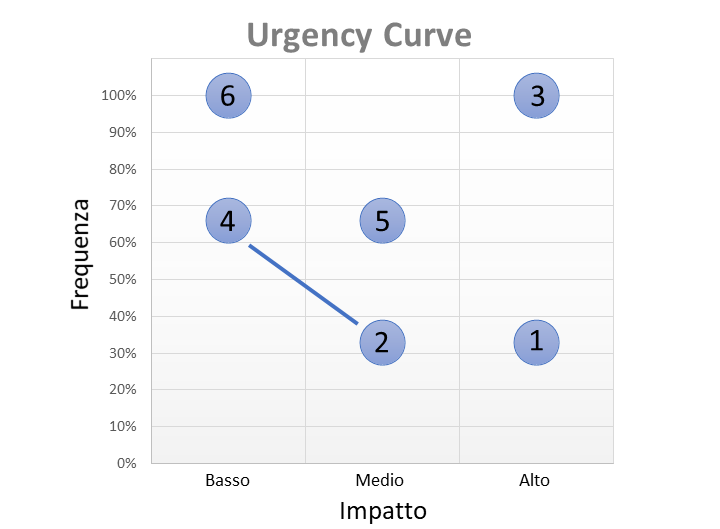
\includegraphics[width=0.6\columnwidth]{valutazione-design/urgency-curve}
    \caption{Curva delle urgenze.}
    \label{fig:testing-urgency-curve}
\end{figure}
\noindent

Le soluzioni adottate per ogni problema sono documentate nel blocchi di iterazione riportati nella \hyperref[s:wireframe]{Sezione 4.6} in cui sono trattati i wireframe: abbiamo deciso di riportare in tali blocchi tutti i raffinamenti e le correzioni apportate seguitamente all'inspection e al testing, al fine di concentrare in un'unica sezione del report l'intera storia evolutiva di ogni componente grafica.